\chapter[Resultados Obtidos]{Resultados Obtidos}

Este capítulo visa relatar os resultados obtidos em ambos os experimentos
realizados para verificar a validades das hipóteses propostas neste trabalho.
Dessa forma, cada experimento será analisado em uma sessão própria.

\subsection{Primeiro Experimento}

A primeira coleta do primeiro experimento foi realizada com 16 pessoas, onde
elas concordaram com os termos do Anexo D. Neste experimento foram analisados
três estratégias de recomendação, sendo elas:

\begin{itemize}
    \item \textbf{cbh:} Estratégia baseada em conteúdo, onde metade do
    perfil do usuário é formado por debtags e a outra metade por termos
    da descrição dos pacotes, tanto as debtags e os termos são definidos
    utilizando a técnica do TFIDF;
    \item \textbf{cbtm:} Estratégia baseada em conteúdo utilisando o contexto
    temporal, assim como na estratégia `cbh`, o perfil do usuário é composto
    por duas metades, sendo as debtags e os termos da descrição dos pacotes,
    porém eles são definidos através de dois pesos, sendo o primeiro uma
    análise de quais pacotes foram recentemente utilizados, e o segundo peso
    se trata da utilização do TFIDF;
    \item \textbf{cbml:} Estratégia baseada em conteúdo, onde o perfil do
    usuário é formado tanto por debtags quanto termos, porém não é composto
    por metade de cada um, utilizando esse perfil é realizado a
    recomendação de vários pacotes, então é utilizado o algoritmo de
    aprendizado de máquina para identificar quais dentre esses pacotes
    devem ser recomendados.
\end{itemize}

Dentre as estratégias a `cbh` já estava implementada no AppRecommender, e as
estratégias `cbtm` e `cbml` se tratam das estratégias implementadas afim de
testar as hipóteses desse trabalho.

Para cada estratégia foram selecionadas as 10 melhores recomendações
e essas foram ordenadas em ordem alfabética e apresentadas uma a uma para
o usuário realizar a pontuação, como foi descrito anteriormente.

A coleta de dados apresentou os resultados apresentados na figura
\ref{fig:primeiro_experimento}

\pagebreak

\begin{figure}[h]
  \centering
  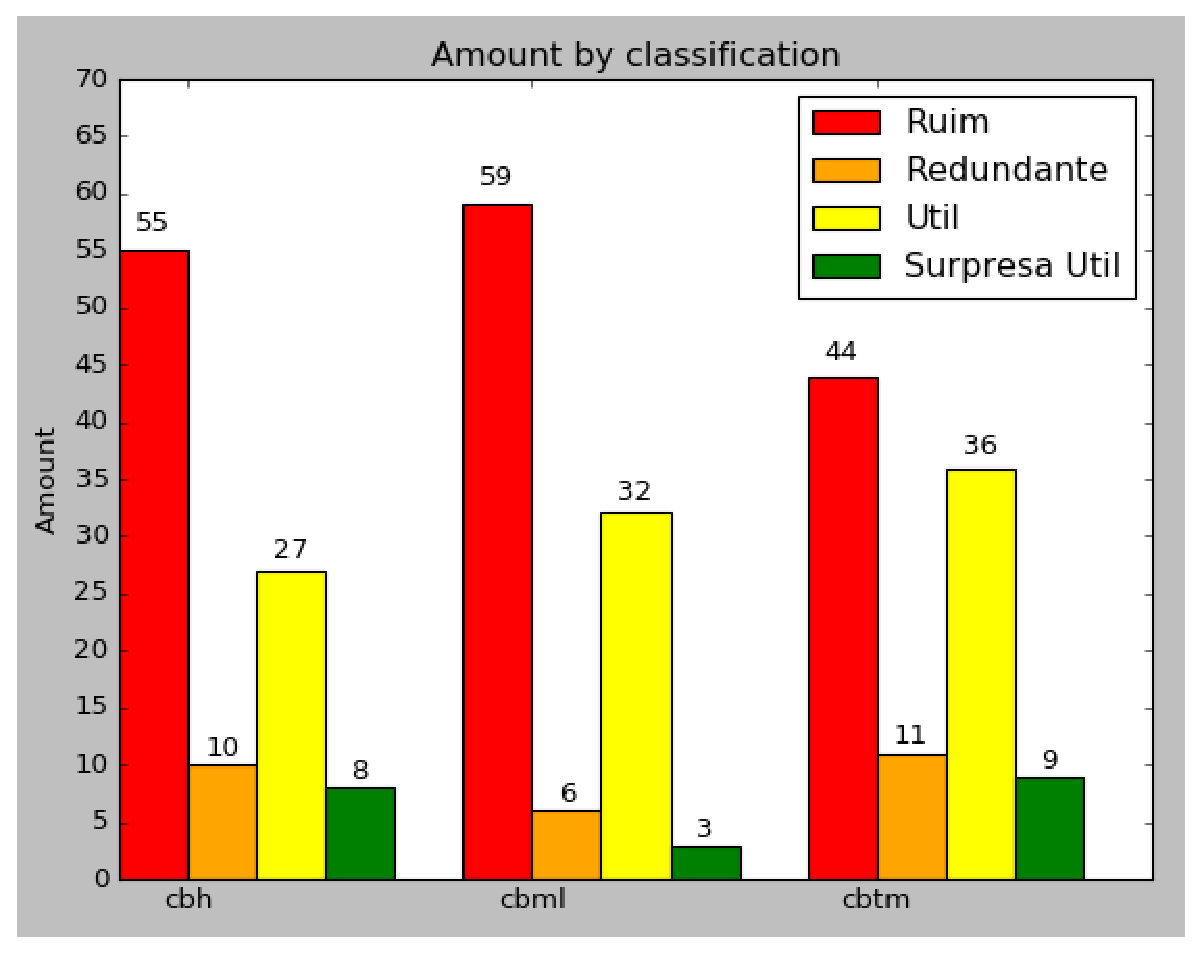
\includegraphics[width=0.9\textwidth]{figuras/primeiro_experimento.eps}
  \caption{Resultados do primeiro experimento}
  \label{fig:primeiro_experimento}
\end{figure}

Analisando os dados coletados pode-se observar que os indices de recomendações
ruins das estratégias `cbh` e `cbml` foram maiores que os indices da estratégia
`cbtm`, e também é notável a diferença entre recomendações úteis e surpresas
boas, pois a estratégia `cbtm` possui 45 recomendações nessas classificações
enquanto as estratégias `cbml` e `cbh` possuem 35.

Através dos dados coletados observa-se que mesmo a estratégia `cbtm` possuindo
um pouco de destaque, todas as estratégias aprensentaram um índice muito alto
de recomendações ruins

Através desses dados coletados realizou-se uma análise das métricas propostas
no Anexo D, a figura \ref{fig:metricas_segundo_experimento} apresenta os valores
das métricas.

\pagebreak

\begin{figure}[h]
  \centering
  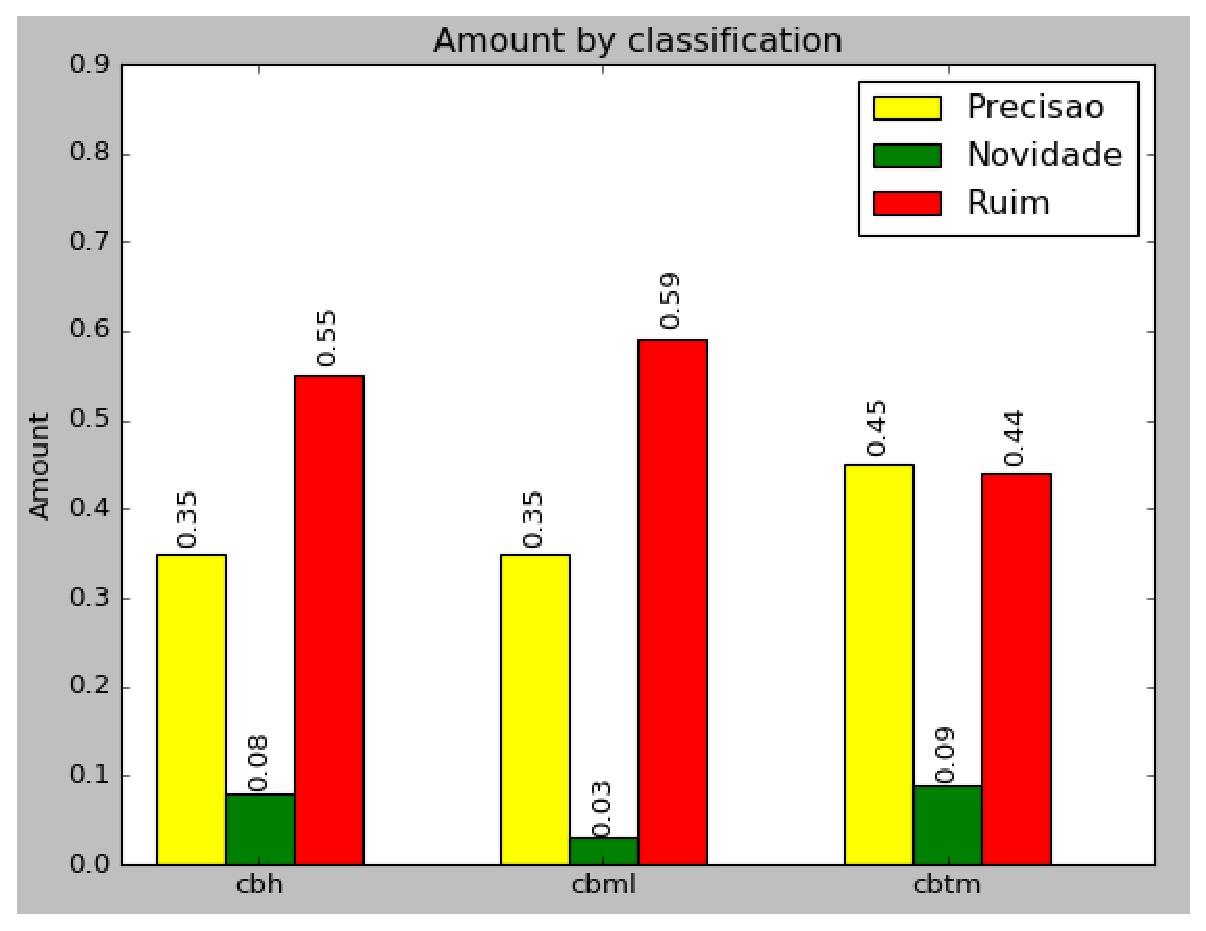
\includegraphics[width=0.9\textwidth]{figuras/metricas_primeiro_experimento.eps}
  \caption{Métricas do primeiro experimento}
  \label{fig:metricas_primeiro_experimento}
\end{figure}

Analisando a precisão e a novidade de cada recomendação, observa-se que a
estratégia que apresentou melhores resultados embora por pouca diferença,
foi a estratégia `cbtm`, fato que pode demonstrar que a estratégia
determinística se saiu melhor que a estratégia de aprendizado de máquina, para
esses usuários que participaram do experimento.

Outra informação coletada no experimento foi a validação cruzada, onde a
figura \ref{fig:primeiro_experimento_cross_validation} apresenta as a média
das métricas coletadas da validação cruzada de cada usuário.

Analisando os gráficos da figura \ref{fig:primeiro_experimento_cross_validation}
observa-se que a unica métrica que está acima de 50\% é a acurácia, o que
indica que o algoritmo de aprendizagem de máquina, ou o tratamento de dados,
como a definição do perfil do usuário, podem ser melhorados afim de que os
resultados dessas métricas possam ser melhorados.

\pagebreak

\begin{figure}[h]
  \centering
  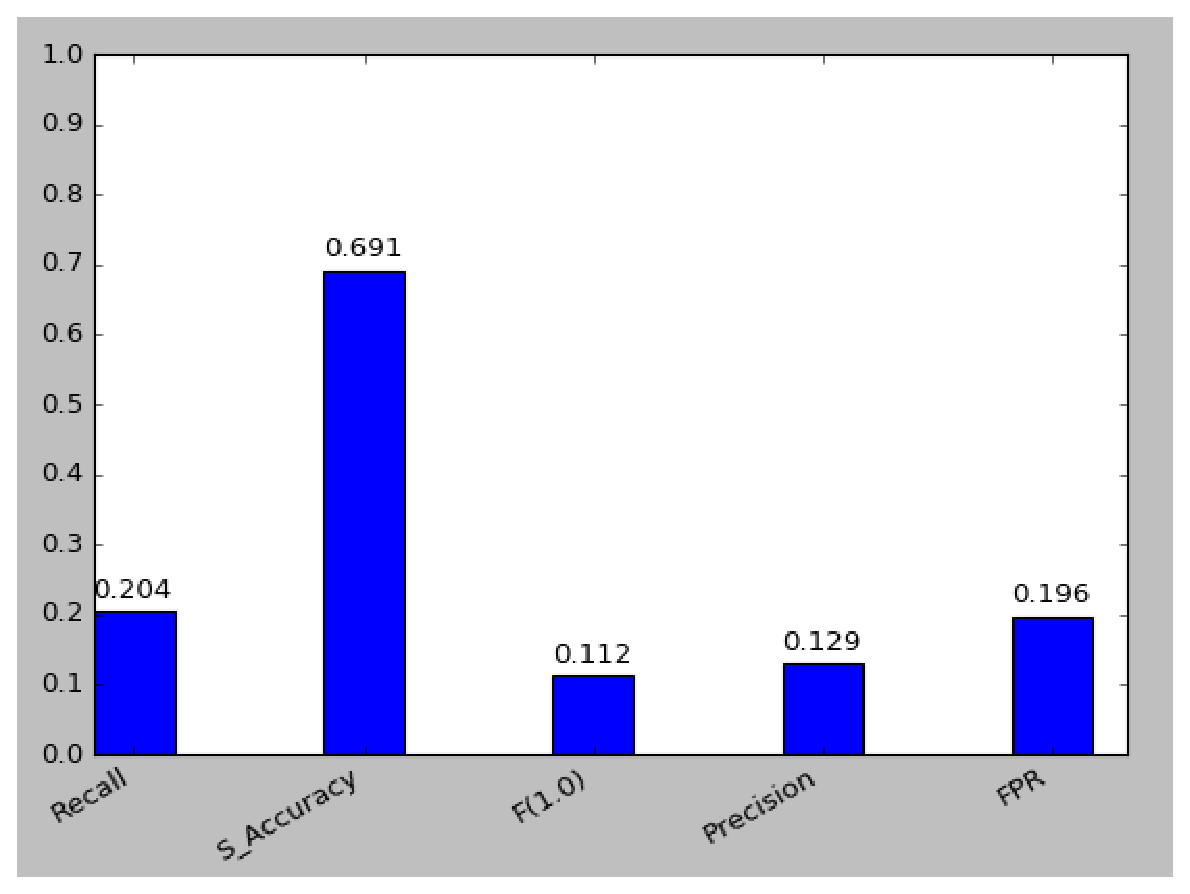
\includegraphics[width=0.9\textwidth]{figuras/primeiro_experimento_cross_validation.eps}
  \caption{Métricas obtidas através da validação cruzada dos usuários que
  participaram do experimento}
  \label{fig:primeiro_experimento_cross_validation}
\end{figure}

Os resultados desse primeiro experimento não foram o que os pesquisadores desse
projeto esperavam, pois esperava-se que os resultados obtidos tivessem um
resultado mais satisfatório quanto a qualidade das recomendações, porém, esse
primeiro experimento foi executado com o objetivo de coletar dados afim de
compreender mais sobre o perfil dos usuários e o que estava sendo recomendado,
e então utilizar isso para melhorar o sistema de recomendação e posteriormente
realizar um segundo experimento onde de fato o objetivo é comparar qual
estratégia se saiu melhor.

\section{Segundo experimento}

Dado os resultados do primeiro experimento, as seguinte medidas foram tomadas
para o segundo experimento:

\begin{itemize}
   \item \textbf{Mudar cálculo do contexto temporal de um pacote: } Visto que
   pelo primeiro experimento, o contexto temporal do pacote não estava
   refletindo bem os usos do usuário, o cálculo do contexto temporal de um
   pacote foi atualizado. O contexto temporal de um pacote agora é calculado de
   forma semelhante ao obtido pelo \textit{popularity-contest}, onde o tempo de
   acesso de cada arquivo relacionado a um pacote é observado e o maior tempo
   encontrado é considerado o tempo de acesso.

   \item \textbf{Balancear rótulo dos pacotes: } Com o intuito de melhorar os
   a acurácia dos algoritmos de aprendizado de máquina, resolveu-se melhor
   balancear os pacotes do usuário. Para isso, os pacotes são ordenados pelo seu
   contexto temporal e dividos em três grupos de igual tamanho, onde cada grupo
   representa um rótulo possível.

   \item \textbf{Selecionar pacotes apenas instalados diretamente pelo
   \textit{apt}:} Para melhorar o perfil de usuário, resolveu-se selecionar não
   mais os pacotes marcados como manualmente instalados pelo sistema, e sim
   apenas aqueles cujo usuário instalou diretamente pelo \textit{apt}.

   \item \textbf{Implementar nova forma de representar um pacote: } Para
   verificar se outras formas de representação de um pacote podem ser mais
   eficientes, implementou-se uma nova estratégia de aprendizado de máquina, que
   usa o modelo \textit{bag of words} juntamente com o \textit{tfidf} para
   representar um pacote.

   \item \textbf{Uso da estratégia de expansão de query: } Essa estratégia já
   implementada pelo \textit{AppRecommender} faz com que o \textit{Xapian}
   apenas receba os pacotes que deva fazer a pesquisa relacionada e o mesmo deve
   entar ser capaz de retirar de cada pacote as informações mais importantes
   para realizar a pesquisa. Dessa forma, as estratégias de aprendizado de
   máquina também foram combinadas com essa estratégia com o intuito de
   verificar se melhores resultados foram gerados.

   \item \textbf{Diminuir número de pacotes passados para o Xapian:} Para as
   estratégias de aprendizado de máquina, apenas os pacotes marcados como
   \textit{Really Useful} (RU) são passados usados para criar o perfil do
   usuário. Isso se dá pelo fato de tentar reduzir o perfil do usuário e fazer
   com o mesmo seja mais focado nos gostos atuais do usuário.

   \item \textbf{Uso da estratégia \textit{cb} ao invés da \textit{cbml}:} Para
   o primeiro experimento, a estratégia \textit{cbh} foi usada. Entretanto,
   o segundo experimento quis colocar mais foco nos termos dos pacotes e
   não de forma equilibrada como funciona o \textit{cbh}. Dessa forma,
   a estratégia do \textit{AppRecommender} usada para comparação com as
   estratégias de contexto temporal, foi a estratégia \textit{cb}, que usa
   tanto termos do pacote como debtags, mas não garante que as mesmas sejam
   apareçam na mesma quantidade no perfil do usuário.

   \item \textbf{Mudança de nome da estratégia \textit{cbml} para
   \textit{mlbva}:} Como agora existem duas estratégias distintas usando
   aprendizado de máquina, resolveu-se renomear a estratégia \textit{cbml}
   para \textit{mlbva}, que significa \textit{Machine Learning Binary
   Vector Approach}. Esse padrão também é seguido para a estratégia de
   \textit{bag of words}, \textit{mlbow}, que significa \textit{Machine
   Learning Bag Of Words}.
\end{itemize}

Além desses pontos já citados, o segundo experimento também foi realizado com
mais usuários, 24 no total, sendo que os usuários escolhidos também apresentavam
um perfil mais geral quanto ao sistemas operacionais usados, pois para o
primeiro experimento, os usuários eram majoritariamente usuários Debian.

Dito, isso o resultado geral da pesquisa pode ser visto no gráfico
\ref{fig:segundo_experimento}

\begin{figure}[h]
  \centering
  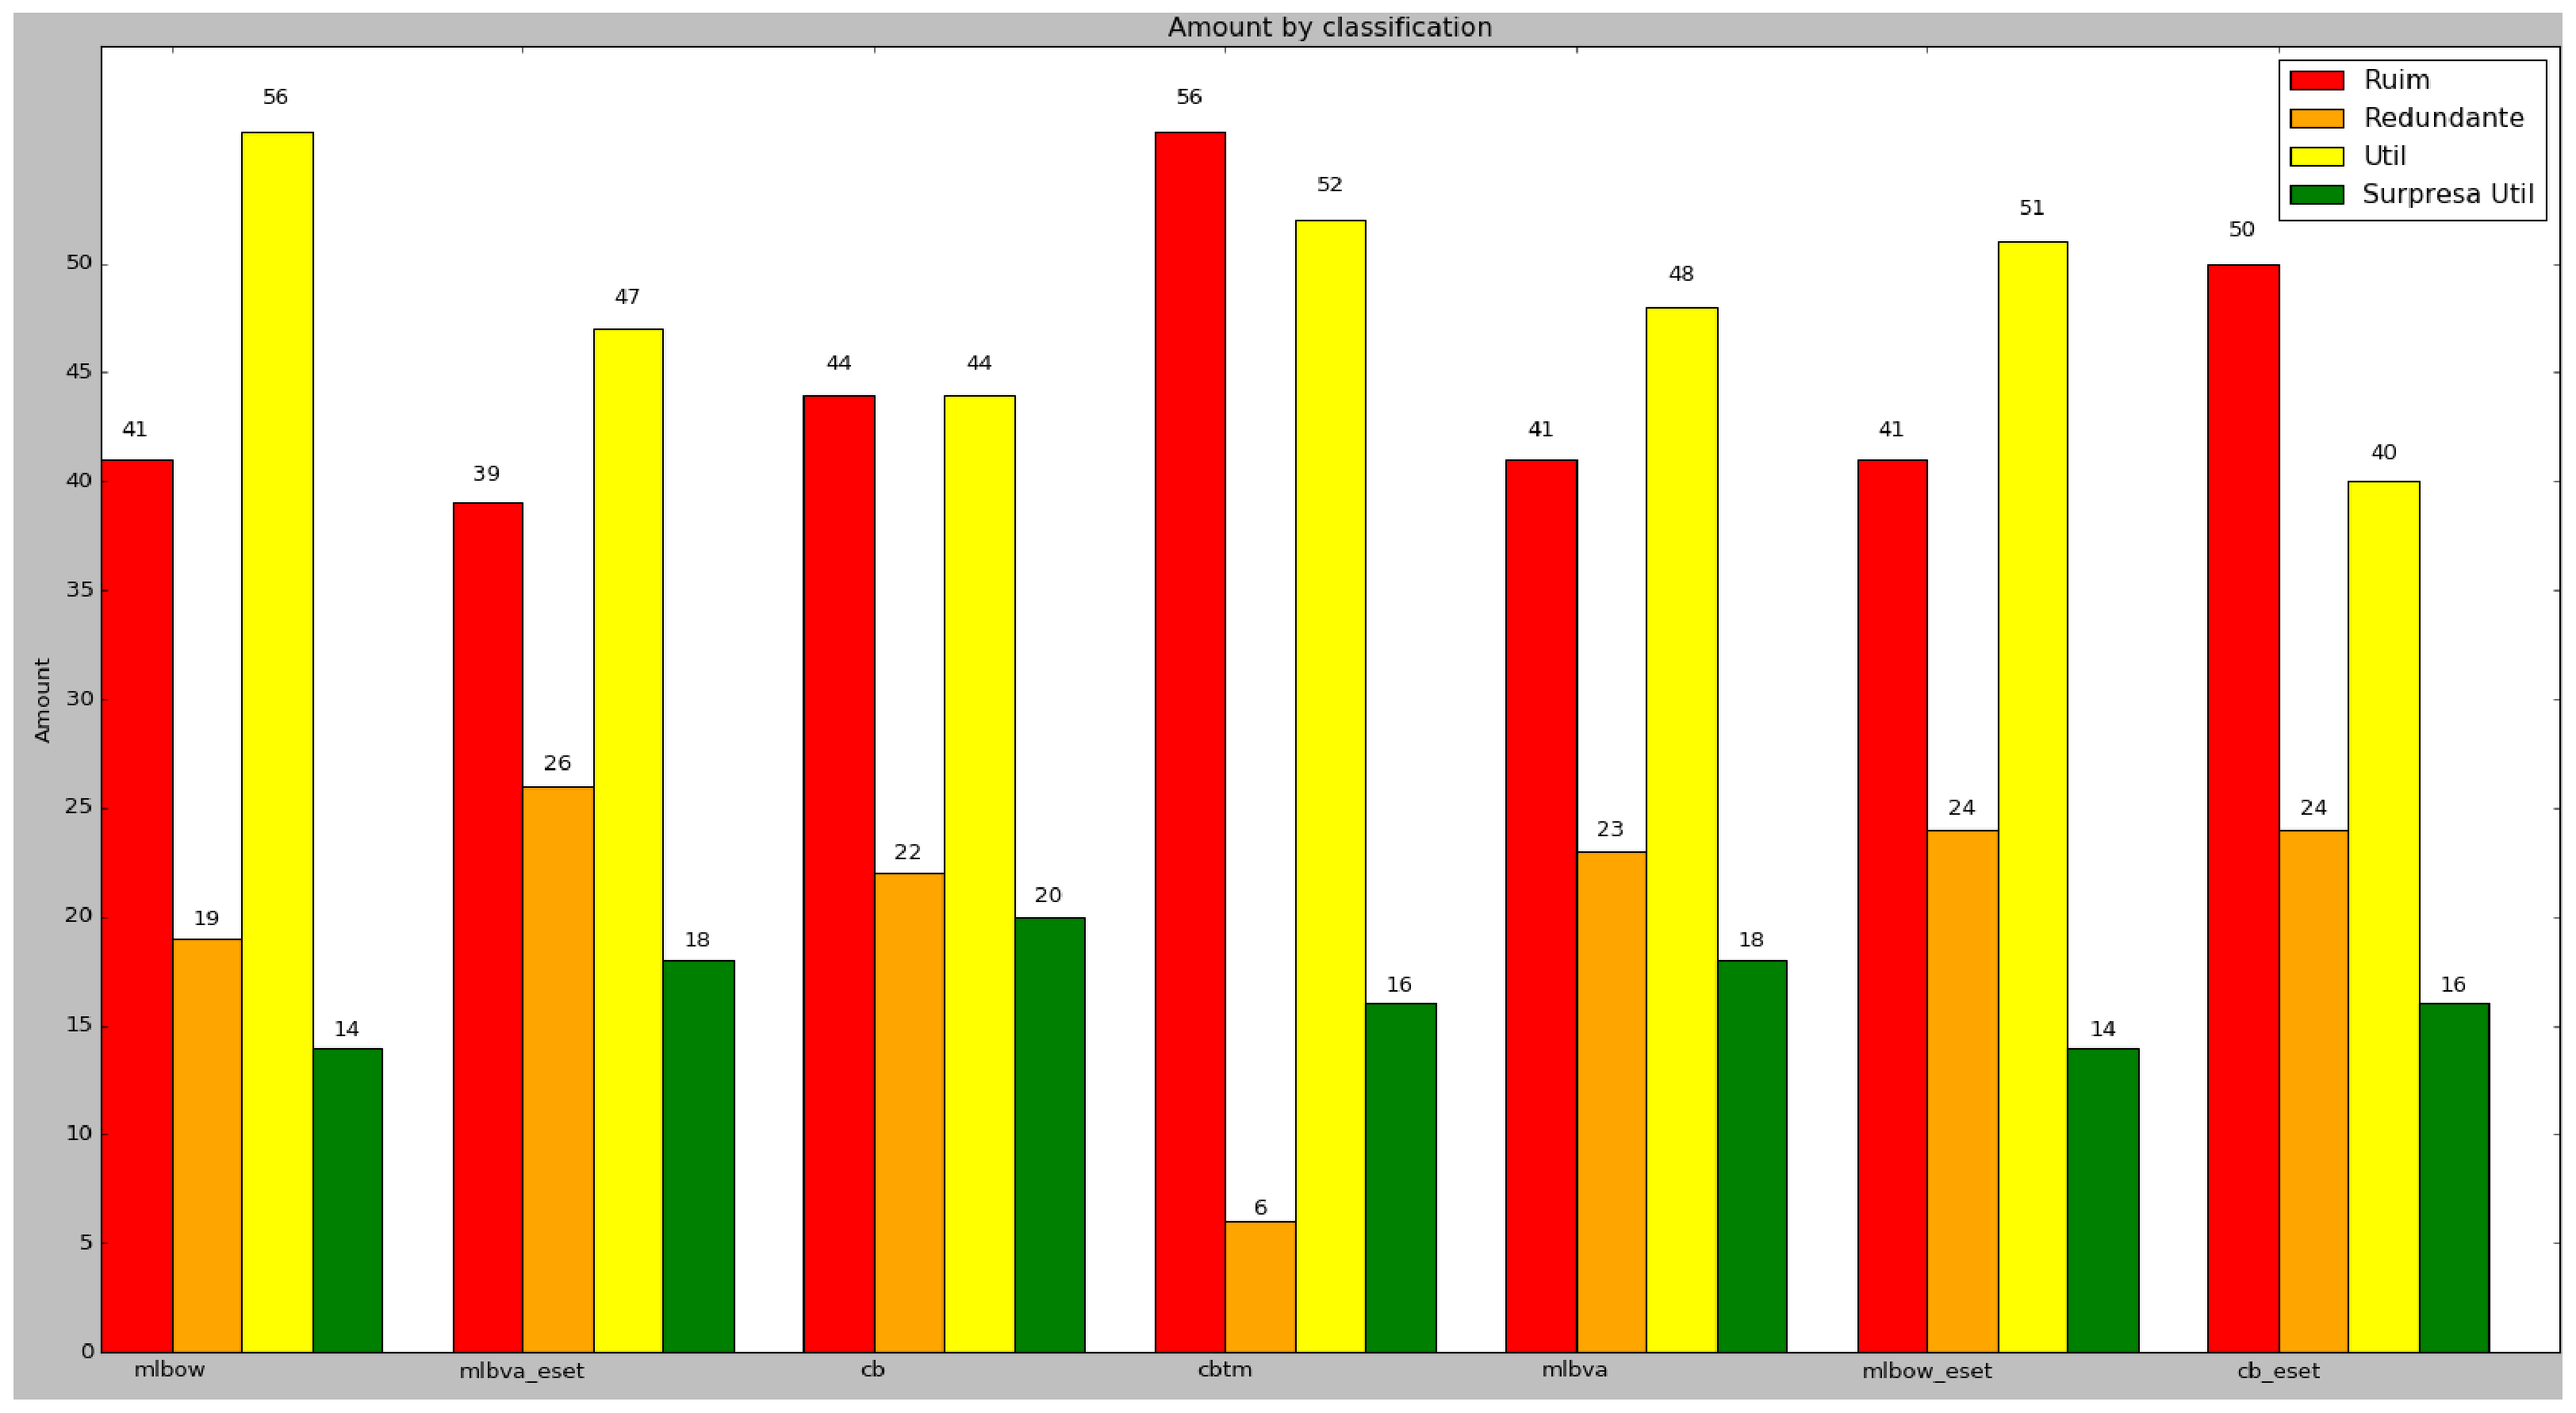
\includegraphics[width=0.9\textwidth]{figuras/segundo_experimento.eps}
  \caption{Resultados do segundo experimento}
  \label{fig:segundo_experimento}
\end{figure}

Para o gráfico \ref{fig:segundo_experimento}, os labels são, respectivamente:

\begin{itemize}
    \item \textbf{mlbow}: Aprendizado de máquina com \textit{bag of words}
    \item \textbf{mlbva\_eset}: Aprendizado de máquina com vetor binário e
    expansão de query.
    \item \textbf{cb}: Estratégia com perfil de usuário sem contexto temporal.
    \item \textbf{cbtm}: Estratégia deterministica com contexto temporal.
    \item \textbf{mlbva:} Aprendizado de máquina com vetor binário.
    \item \textbf{mlbow\_eset:} Aprendizado de máquina com \textit{bag of words}
        usando expansão de query.
    \item \textbf{cb\_eset:} Estratégia usando apenas expansão de query, sem
        contexto temporal.
\end{itemize}

Visualmente, pode-se perceber que apenas as estratégias de aprendizado de
máquina apresentaram um total de recomendações úteis ao usuário maior que o
total de recomendações ruins. Além disso, percebe-se que as estratégias como um
todo estão produzindo poucos resultados considerados uma surpresa para usuário e
estão gerando números próximos de pacotes redundantes.

Uma melhor análise pode ser feita ao observar o gráfico
\ref{fig:metricas_segundo_experimento} com a relação as métricas calculadas para cada
estratégia, conforme definidas na seção de \ref{sec:estudo_usuario}

\begin{figure}[h]
  \centering
  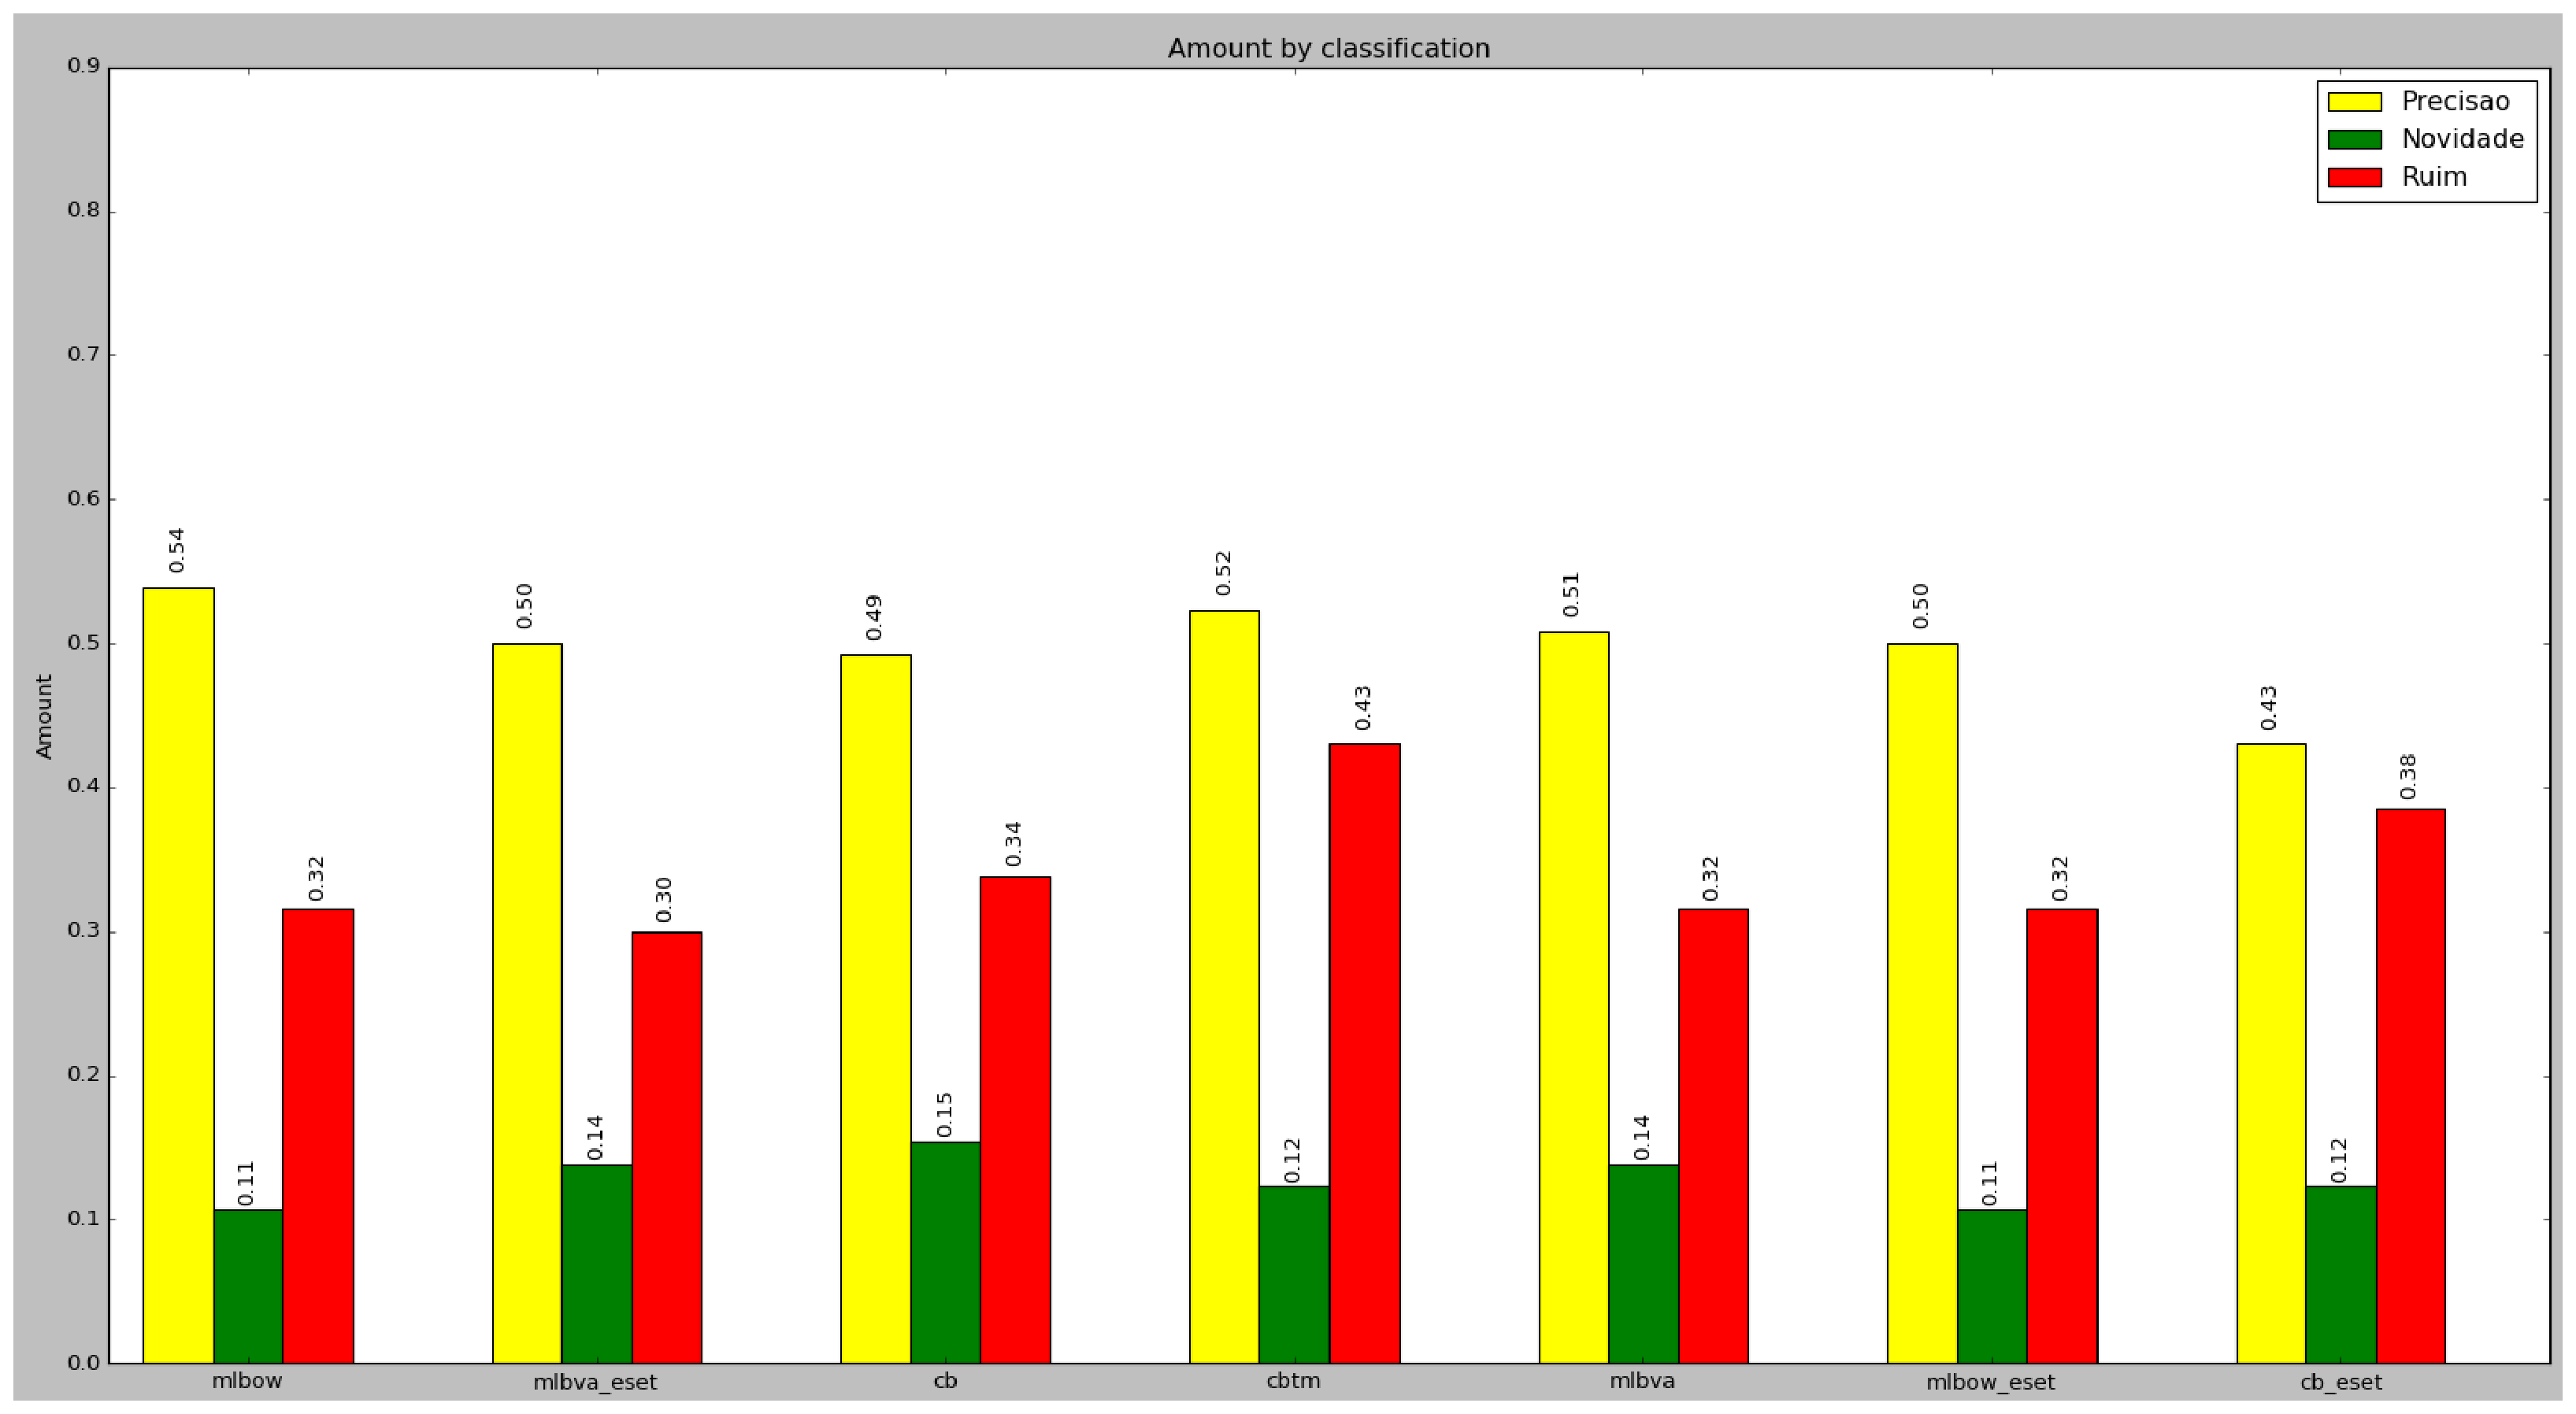
\includegraphics[width=0.9\textwidth]{figuras/metricas_segundo_experimento.eps}
  \caption{Métricas do segundo experimento}
  \label{fig:metricas_segundo_experimento}
\end{figure}

Pode-se ver pelo gráfico \ref{fig:metricas_segundo_experimento} quanto a
precisão, o melhor resultado foi para estratégia \textit{mlbow}. Entretanto, a
melhora se deu em apenas 5\% em relação as estratégias baseada em conteúdo do
\textit{AppRecommender}. Vale ressaltar também que a métrica \textbf{novidade}
mostra o que foi observado no gráfico \ref{fig:segundo_experimento}, onde o
número de recomendações marcadas como surpresa se manteve estável entre as
ferramentas.

Além disso, pode-se perceber que a estratégia determinística com contexto
temporal \textit{cbtm} foi a que recomendou mais pacotes ruins considerados pelo
usuário, ou seja, a estratégia não atende aos requisitos. Isso difere dos
resultados encontrados no primeiro experimento. Percebeu-se então que a mudança
no cálculo temporal favoreceu as estratégias de aprendizado de máquina, mas não
a determinística.

Sobre a questão de redundância, percebeu-se também um problema quanto a pacotes
instalados por outros gerenciadores de pacote. Por exemplo, caso o usuário seja
um programador ruby e tenha instalado pacotes ruby via \textit{apt} e
\textit{Ruby Version Manager} (rvm), o \textit{AppRecommender} pode recomendar
pacote instalados pelo \textit{rvm}, o que causa a redundância.

Por fim, é necessário entender por que a melhoria encontrada foi de 3\%-5\% em
relação as estratégias baseadas em conteúdo já implementadas pelo
\textit{AppRecommender}. O gráfico \ref{fig:segundo_experimento_cross_validation}
mostra a média da métrica de acurácia \textit{PorcentagemAcertos}, definida na seção
\ref{subsec:validacao_cruzada}, para cada estratégia de aprendizado de máquina.
Tal gráfico mostra que nenhuma estratégia teve média muito alta de acurácia, sendo
que acredita-se que a melhora encontrada por essas estratégias foi devido a
pré-filtragem de pacotes e não para a pós filtragem dos mesmos.

\begin{figure}[h]
  \centering
  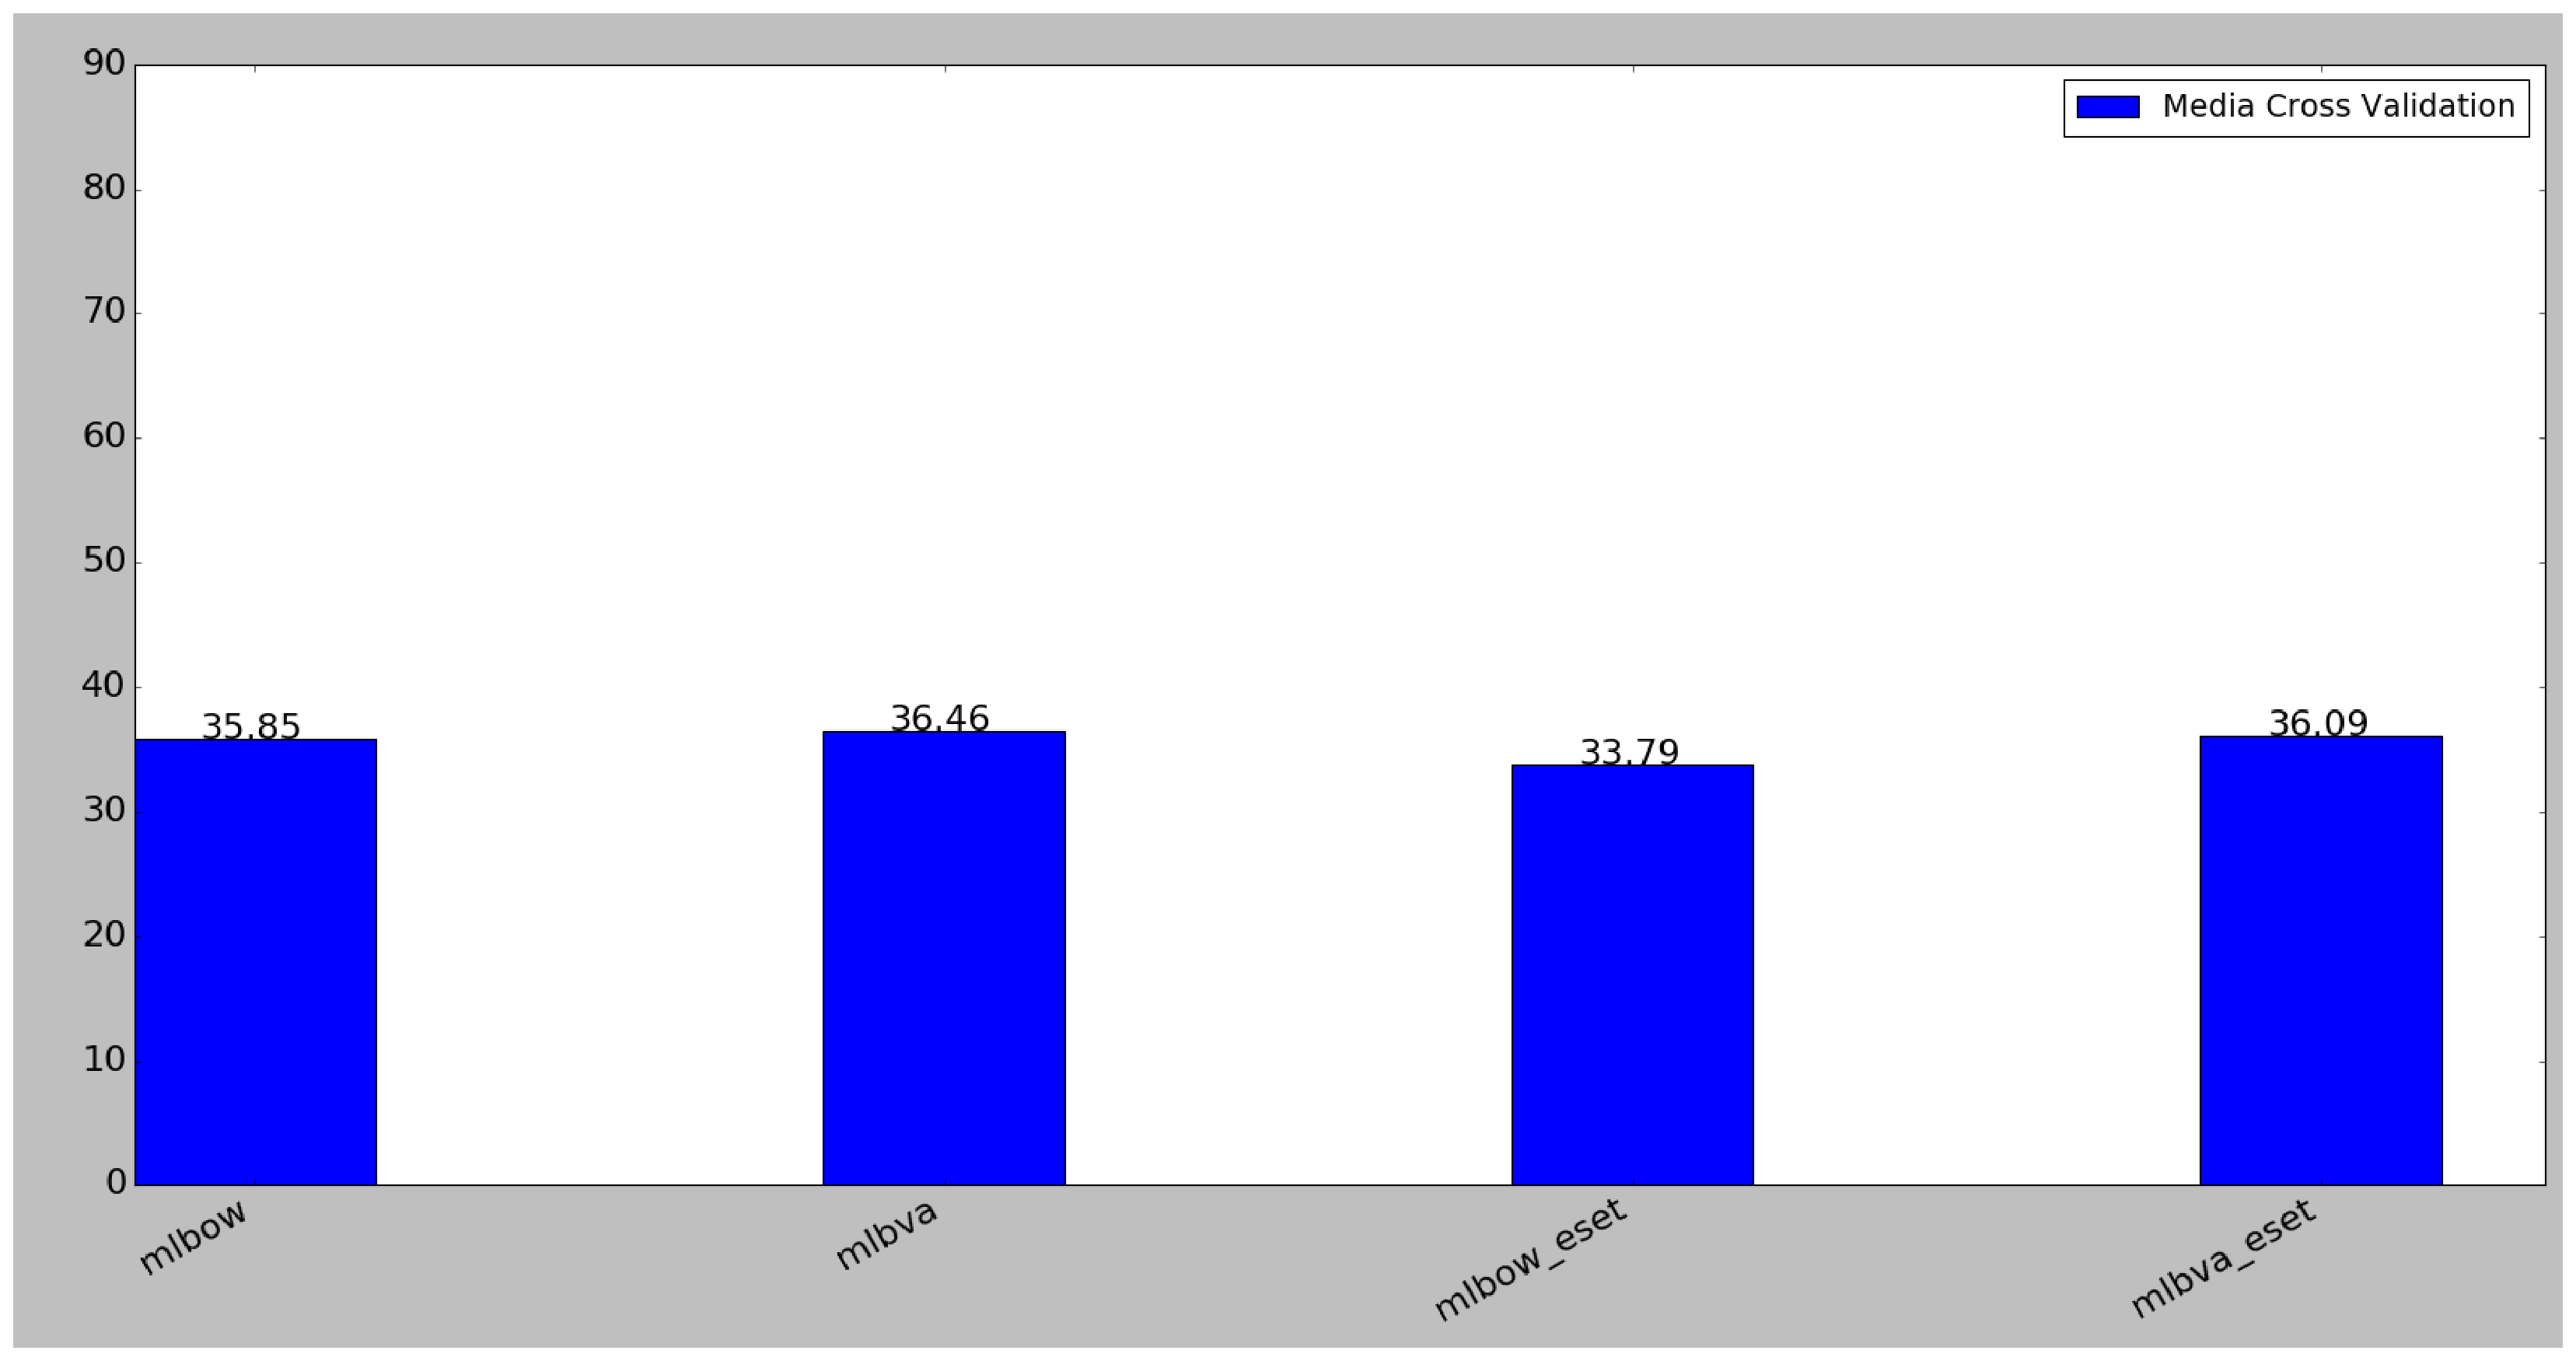
\includegraphics[width=0.9\textwidth]{figuras/segundo_experimento_cross_validation.eps}
    \caption{Métrica \textit{PorcentagemAcertos} obtida via cross validation para cada estratégia de aprendizado de máquina}
  \label{fig:segundo_experimento_cross_validation}
\end{figure}

Vale ressaltar que mesmo com a estratégia de pré-filtragem sendo a que tenha
proporcionado a melhora de resultados, pode-se ver que entre as estratégias de
aprendizado de máquina, as estratégias de classificação também tiveram uma
influência, pois todas as estratégias faziam a pré-filtragem de forma idêntica,
mas foi a \textit{mlbow} com o uso de \textit{bag of words} e \textit{TFIDF} que
se mostrou com melhores resultados.

À partir dessa análise, acredita-se que um dos principais motivos para a baixa acurácia dos algoritmos
se dá pelo número de dados usado pelo treinamento. Em média, apenas 37 pacotes
eram pacotes estavam sendo usados para treinar o algoritmo, o que é uma
quantidade baixa para o treinamento do algoritmo propriamente dito.

Além disso, o método de aprendizado de máquina utilizado, o Bayes ingênuo pode
ser um método muito simples para entender a questão do gosto do usuário e seus
pacotes, sendo que outros métodos poderiam ter sido explorados.
